\appendix
\chapter{Anhang}
	\begin{figure}[h]
		\centering
		\includesvg[width=\textwidth]{Assets/mosfets-Power MOSFETS}
		\caption[Schaltplan der Leistungsendstufe des ESC]{Schaltplan der Leistungsendstufe des ESC\cite{vesc.documentation.2015}.}%
		\label{fig:power mosfets}
	\end{figure}
	\newpage
	\begin{figure}[t]
		\centering
		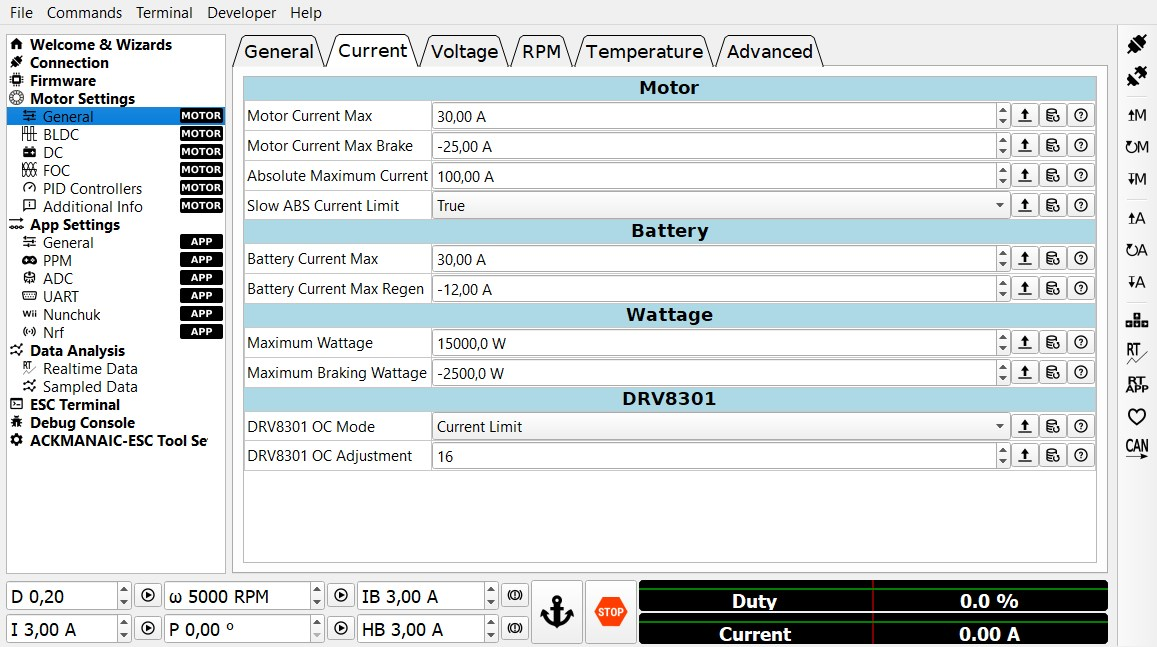
\includegraphics[width=\textwidth]{Assets/ESC_Motor_Parameters.jpg}
		\caption[Testparameter, wie sie in der Konfigurationssoftware der ESC eingetragen wurden]{Testparameter, wie sie in der Konfigurationssoftware der ESC eingetragen wurden und gelten pro Motor. Einträge unter \texttt{Wattage} können ignoriert werden, da nicht verwendet.}%
		\label{fig:ESC motor params}
	\end{figure}
	\begin{figure}[b]
		\centering
		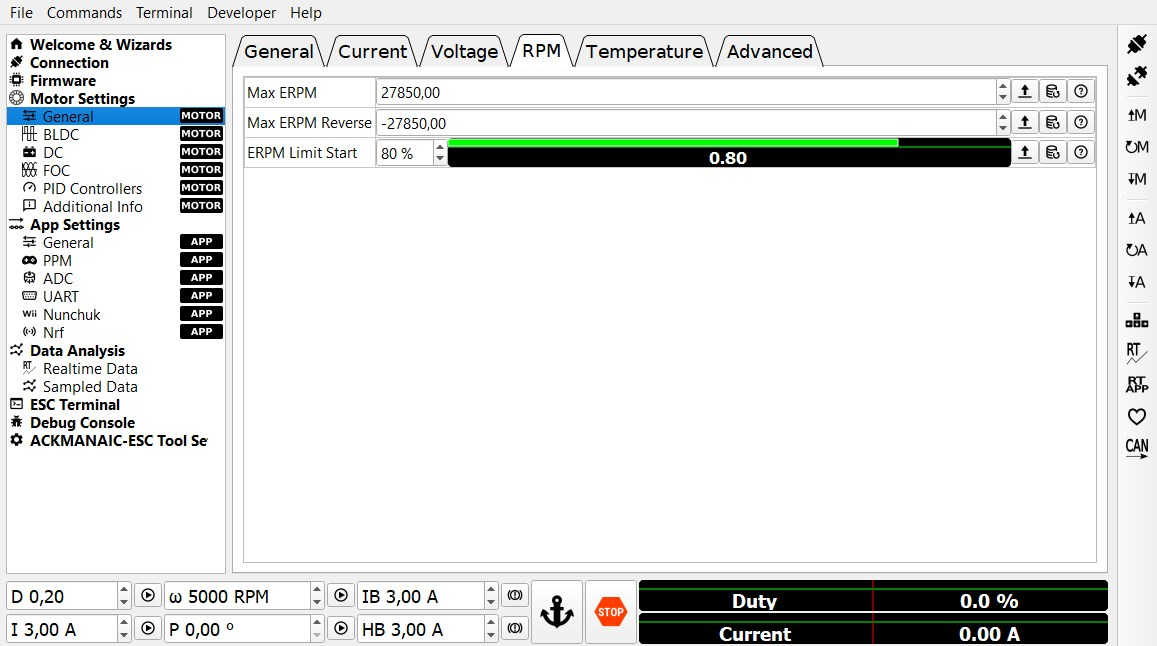
\includegraphics[width=\textwidth]{Assets/ESC_erpm.jpg}
		\caption[In-Software begrenzte elektrische Drehzahl]{In-Software begrenzte elektrische Drehzahl. Hier mit einem Wert von \qty{27850}{\per\minute}.}%
		\label{fig:ESC erpm setting}
	\end{figure}
	\newpage
	\begin{figure}[h]
		\centering
		\includesvg[width=.9\textwidth]{Calc/ESC_testdrive_plot}
		\caption[]{To be captured.}%
		\label{fig:esc testdrive plot}
	\end{figure}